\documentclass{article}

\usepackage{geometry}
\geometry{top=1in,bottom=1in}

\usepackage{tikz}
\usetikzlibrary{positioning}
\usepackage{amsmath}
\usepackage{amsthm}
\usepackage{amssymb}
\tikzset{main node/.style={circle,fill=blue!20,draw,minimum size=1cm,inner sep=0pt},}

\author{Andrew Osborne}
\title{Algorithms Assignment 8}


\begin{document}
  \maketitle

  \section*{Problem 15.2-2}

    The solution to this problem is a simple modification to the already 
    existing \verb Print-Optimal-Parens(s,i,j)   which I will display below

    \begin{verbatim}
      Optimal-Mult(A,s,i,j)
        if i == j
          return A[i]
         else
          // assuming matrix multiplication is already implemented
          return Optimal-Mult(A,s,i,s[i,j])*Optimal-Mult(A,s,s[i,j]+1,j)
    \end{verbatim}  

  \section*{Problem 22.2-9}
    
    Now, let us suppose that \verb G  is a graph with edges and vertices
    and that we have access to the \verb BFS(G,s)  which is written in the text.
    Firstly, let us denote the edge between nodes \verb u  and \verb  v by 
    \verb E(u,v)  and let us further suppose that we may store such objects
    in an array.
    Then, in the syntax of the book's pseudocode, our algorithm is given by 

    \begin{verbatim}
      BFS(G,s) // now every node but s has non-null pi value
      Assign to each vertex in G a distinct integer .id value
      let V be an empty vector of edges

      DoublePath(G,V,s)
        for each vertex u in G.adj[s]
          if u.pi == s // hits each node exactly once
            V.append(E(s,u))
            DoublePath(G,V,u)
          else if s.id < u.id // hits at most 2*E times 
            V.append(E(s,u))
            V.append(E(u,s))
    \end{verbatim}
    With \verb BFS  , we are constructing a tree with \verb s  at the root
    and our recursion ensures that all paths in said tree are traversed
    exactly once in each direction, and the other appendation accounts for 
    those paths which are pruned by BFS. 
    Note that we need the \verb .id  values because we would otherwise 
    traverse each pruned edge twice in each direction, rather than once.
    \verb BFS  runs in $O(E + V$$)$ time and our recursion runs in 
    $$\Theta(V) + O(E + V) + O(E + V) = O(E + V)$$
    time.

  \section*{22.3-1}
    In the following tables, let C denote cross edges, T denote tree edges, F denote forward edges, and B denote back edges.
    Furthermore let ``-" indicate that there are no valid edges. 
    Finally $A[i,j]$ represents the valid edges between color i and color j.
    \begin{center}
      For Directed Graphs \\
    \begin{tabular}{|c|c|c|c|}
      \hline                    
       - & Black & White & Gray \\
      \hline                    
      Black & all & - & B       \\
      \hline                    
      White & C & all & CB      \\
      \hline                    
      Gray & FCT & T & BFT      \\
      \hline 
    \end{tabular}
    \end{center}
    
    \begin{center}
      For Undirected graphs \\
      \begin{tabular}{|c|c|c|c|}
      \hline
      - & Black & White & Gray \\ \hline
      Black & TB & - & B \\ \hline
      White & - & TB & B \\ \hline
      Gray  & T & T & TB \\ \hline
      \end{tabular}
    \end{center}
  \section*{22.3-7}
    This problem will be answered almost exclusively with pseudocode because of 
    the simplicity of the problem.
    Let us assume that we possess a stack data structure which has \verb pop()  which
    removes and returns the top element of the stack,
    \verb peek()  which returns but does not remove the object on the top of the 
    stack and \verb push(v)  which pushes \verb v  onto the top of the stack.
    Finally assume our stack datastructure has a \verb hasNext()  field which 
    returns true if and only if \verb pop()!=NIL  .
    \begin{verbatim}
      DSF(G)
        for each vertex v in G.V
          v.pi = NIL
          v.color = white
        time = 0
        let S be an empty stack of vertices
        
        for each vertex v in G.V
          if v.color == white
            time += 1
            v.color = gray
            v.d = time
            S.push(v)
            while S.hasNext()
              // updates peek() going depth first
              // if we pass this loop, we arrived at 
              // a node with no white descendants
              for vertex u in G.adj[S.peek()]
                if u.color == white
                  time += 1
                  u.color = gray
                  u.pi = S.peek()
                  u.d = time
                  S.push(u)
              time = time + 1
              x = S.pop()
              x.color = black
              x.f = time
    \end{verbatim}
    This algorithm is identicle in nature to the one in the text.
    Note that the peek() function is particularly important here. 
    Also note that in the innermost for loop, when I push an element to S, 
    that element will be returned as S.peek() in future iterations.
    The innermost for-loop will only exit when a node with no white children is 
    found, at which point we will pop said element off of the stack, color it black,
    declare it finished, and proceed in this way until S is empty. 

  \section*{22.3-8}
  \begin{center}
    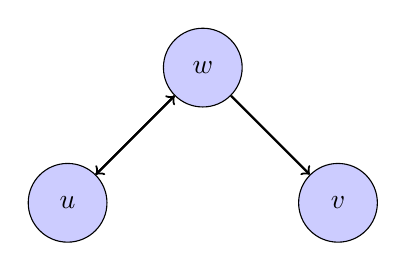
\begin{tikzpicture}
      \node[main node] (1) {$w$};
      \node[main node] (2) [below left = 1cm and 1cm of 1]{$u$};
      \node[main node] (3) [below right = 1cm and 1cm of 1]{$v$};

      %\draw[edge] (1) to (2)
      %\draw[edge] (1) to (3)
      %\draw[edge] (2) to (1)

      \path[draw,thick][->]
        (1) edge node {} (2)
        (1) edge node {} (3)
        (2) edge node {} (1);

    \end{tikzpicture}
  \end{center}
  Clearly, in the above graph, there is a path from $u$ to $v$ which is identically
  $u \to w \to v$ but if we begin our DFS on w, discover u, and then discover v, we have 

  \begin{center}
  \begin{tabular}{|c|c|c|}
    \hline
    node & d & f \\ \hline
    w & 1 & 6    \\ \hline
    v & 4 & 5    \\ \hline
    u & 2 & 3    \\ \hline
  \end{tabular}
  \end{center}
  This is sufficient for a counterexample to the proposed conjecture.

\end{document}
